\documentclass[a4paper,11pt]{article}

\usepackage[T1]{fontenc}
\usepackage[utf8]{inputenc}
\usepackage[brazilian]{babel}
\usepackage{graphicx}
\usepackage{booktabs}
\usepackage{geometry}
\usepackage{hyperref}
\usepackage{amsmath}
\usepackage{float}
\usepackage{natbib}

\geometry{margin=2.5cm}
\hypersetup{colorlinks=true, linkcolor=black, citecolor=black, urlcolor=black}
\graphicspath{{../figures/}}

\title{AutoML para Previsão da Produção de Arroz na América do Sul \\
\large Atividade Prática 1, SCC0233: Aplicações de Aprendizado de Máquina e Mineração de Dados}
\author{Renato Spessotto, 14605824}
\date{30 de agosto de 2026}

\begin{document}
\maketitle

\begin{abstract}
\noindent Este relatório revisita o problema de previsão da produção anual de arroz
na América do Sul estudado por \citet{grion2026rice}. A configuração manual de modelos
(Regressão Linear, SVR e XGBoost) foi substituída por AutoML com o AutoGluon-Tabular
\citep{erickson2020autogluon}. Com os mesmos dados (FAOSTAT e NASA POWER) e os mesmos
cenários do artigo, o AutoGluon superou o XGBoost manual em três dos quatro cenários:
MAPE de 7,20\% contra 13,72\% no holdout agrícola, e de 5,05\% e 6,55\% contra 12,47\% e
11,30\% na validação cruzada. No quarto cenário, o holdout com clima, ficou empatado com o
XGBoost (8,99\% contra 8,79\%, valor aproximado). O relatório também abre a caixa-preta:
mostra a composição do ensemble, o erro de teste de cada modelo, a importância dos
atributos, a sensibilidade ao preset e ao tempo, a variação entre sementes e o custo
computacional.
\end{abstract}

\section{Introdução}

O artigo de referência \citep{grion2026rice}, ``Predictive Modeling of Rice
Production in South America Using Machine Learning'' (SBSI 2026), prevê a produção
anual de arroz em 12 países da América do Sul a partir de dados agrícolas da
FAOSTAT \citep{faostat2025} e climáticos da NASA POWER \citep{nasapower2018}.
Ele compara Regressão Linear, SVR e XGBoost configurados manualmente e aponta o XGBoost
como o modelo mais equilibrado, com MAPE entre aproximadamente 9\% e 14\%, conforme o
cenário.

O objetivo desta atividade é investigar se uma abordagem de AutoML consegue
resultados competitivos com os do estudo de referência, automatizando a seleção de
algoritmo e o ajuste de hiperparâmetros, sem tratar a ferramenta como caixa-preta.
Todo o código, as tabelas e as figuras deste relatório foram gerados no notebook
\texttt{rice\_automl.ipynb}, entregue junto com este documento.

\section{Trabalho de referência}

O estudo original usa dados da FAOSTAT (2004 a 2023) e da NASA POWER (2011 a 2023)
para os 12 países da América do Sul. Os atributos são \textit{Area harvested (ha)} e
\textit{Yield (kg/ha)} e, na versão com clima, a temperatura média e a precipitação
anuais; o alvo é \textit{Production (t)}. Os autores testam janelas de treino de 5,
10 e 15 anos e concluem que 10 anos oferecem o melhor equilíbrio entre abrangência e
atualidade. Os resultados usados aqui como referência estão na
Tabela~\ref{tab:baseline-artigo}.

\begin{table}[H]
\centering
\caption{MAPE (\%) reportado no artigo original, por cenário e modelo.}
\label{tab:baseline-artigo}
\begin{tabular}{@{}llrrr@{}}
\toprule
Cenário & Atributos & Regressão Linear & SVR & XGBoost \\
\midrule
Holdout 3 anos (2021--2023) & agrícolas & 32,38 & 121,15 & 13,72 \\
Holdout 3 anos (2021--2023) & + clima & 2,13\textsuperscript{*} & 13,00\textsuperscript{*} & 8,79\textsuperscript{*} \\
Validação cruzada $k=5$ & agrícolas & 34,87 & 137,23 & 12,47 \\
Validação cruzada $k=5$ & + clima & 34,60 & 121,00\textsuperscript{\dag} & 11,30 \\
\bottomrule
\end{tabular}
\\[2pt]
\footnotesize{\textsuperscript{*}Valores aproximados a partir do texto do artigo, que
não publica um MAPE agregado de 3 anos para o cenário com clima. Regressão Linear: média
dos erros anuais de 2021, 2022 e 2023 (0,76\%, 3,94\% e 1,69\%). XGBoost: média de 4,37\%
(2021) com os valores de 2022 e 2023, descritos apenas como ``cerca de 11\%''. SVR: ponto
médio da faixa de erro relatada para o período (9\% a 17\%), sem valor pontual por ano. \\
\textsuperscript{\dag}O artigo relata apenas que o SVR na validação cruzada com
clima ``superou 120\%'', sem publicar o valor exato; 121,00 é usado aqui como
aproximação para permitir a comparação numérica.}
\end{table}

\section{Configuração experimental}

Usamos o dataset que já integra FAOSTAT e NASA POWER, do repositório oficial do artigo
\citep{grion2026repo} (\texttt{dataset\_NASA\_FAOSTAT.csv}): 12 países no período de 2011
a 2023, num total de 156 observações, sem valores ausentes.

\paragraph{Ferramenta.} Escolhemos o AutoGluon-Tabular \citep{erickson2020autogluon} por três motivos:
\begin{itemize}
  \item treina uma família ampla de modelos: LightGBM, CatBoost, XGBoost, Random Forest,
  Extra Trees, KNN, redes neurais e modelos lineares;
  \item combina esses modelos com \textit{bagging} em $k$ folds e \textit{stack
  ensembling} em várias camadas. Num dataset pequeno, isso garante que cada modelo seja
  avaliado fora da amostra;
  \item oferece ferramentas de inspeção: um \textit{leaderboard} com o erro de validação e
  de teste de cada modelo, os pesos do ensemble, os hiperparâmetros e a importância por
  permutação.
\end{itemize}

\paragraph{Cenários.} Replicamos os dois eixos centrais de comparação do artigo original:

\begin{itemize}
  \item \textbf{Cenário A, holdout temporal:} treino em 2011--2020, teste em 2021--2023,
  sem e com variáveis climáticas.
  \item \textbf{Cenário B, validação cruzada $k=5$:} sobre 2011--2023, também sem e com
  clima, reportando o MAPE médio e o desvio-padrão entre folds.
\end{itemize}

\paragraph{Configuração do AutoGluon.} Cada execução treina um \texttt{TabularPredictor} do
zero com:
\begin{itemize}
  \item \texttt{eval\_metric="mean\_absolute\_percentage\_error"}, otimizando diretamente a
  métrica do artigo;
  \item \texttt{presets="best\_quality"};
  \item 120\,s de orçamento no Cenário A e 60\,s por fold no Cenário B.
\end{itemize}
A variável \texttt{Pais} entra como categórica, e o pré-processamento fica a cargo da
ferramenta. O preset e o tempo foram escolhidos por um estudo de sensibilidade
(Seção~\ref{sec:sensibilidade}). Para medir a variabilidade, o Cenário A foi repetido com
três sementes (42, 7 e 2026). Reportamos o MAPE (Eq.~\ref{eq:mape}), obrigatório, e
também MAE, RMSE e R\textsuperscript{2}.

\begin{equation}
\text{MAPE} = \frac{100\%}{n}\sum_{i=1}^{n}\left|\frac{y_i - \hat{y}_i}{y_i}\right|
\label{eq:mape}
\end{equation}

\section{Resultados}

\subsection{Processo do AutoML}

Nos dois conjuntos de atributos, o modelo final foi um \texttt{WeightedEnsemble\_L3}: uma
média ponderada, com pesos ajustados nas predições \textit{out-of-fold}, de modelos de duas
camadas de \textit{stacking}. A Tabela~\ref{tab:leaderboard} mostra os principais modelos do
\textit{leaderboard}, com o MAPE de validação, que guiou a seleção, e o de teste, que só foi
calculado depois.

\begin{table}[H]
\centering
\caption{Leaderboard do AutoGluon no Cenário A (agrícola), ordenado pela validação. Em negrito, o modelo selecionado.}
\label{tab:leaderboard}
\begin{tabular}{@{}lcrr@{}}
\toprule
Modelo & Camada & MAPE validação (\%) & MAPE teste (\%) \\
\midrule
\textbf{WeightedEnsemble\_L3} & 3 & \textbf{4,34} & \textbf{7,20} \\
WeightedEnsemble\_L2 & 2 & 4,41 & 6,89 \\
RandomForestMSE\_BAG\_L2 & 2 & 5,24 & 8,93 \\
ExtraTreesMSE\_BAG\_L1 & 1 & 5,49 & 8,65 \\
RandomForestMSE\_BAG\_L1 & 1 & 8,18 & 11,67 \\
NeuralNetTorch\_BAG\_L1 & 1 & 8,51 & 25,44 \\
XGBoost\_BAG\_L1 & 1 & 8,68 & 10,01 \\
CatBoost\_BAG\_L1 & 1 & 15,26 & 18,84 \\
\bottomrule
\end{tabular}
\end{table}

\paragraph{Composição do ensemble.} No cenário agrícola, o ensemble final dá 56\% do peso a
um Extra Trees com \textit{bagging}, 19\% a uma rede neural, 12\% a um Random Forest da
camada 2 e 6\% cada a LightGBM e CatBoost. Com clima, o Extra Trees fica com 36\%, o Random
Forest da camada 2 com 32\%, uma rede neural com 20\% e o CatBoost com 12\%. Os
hiperparâmetros do Extra Trees são os padrões da ferramenta (300 árvores,
\texttt{max\_leaf\_nodes}=15000). O ganho vem da combinação de modelos, não de uma busca
fina de hiperparâmetros.

\paragraph{Validação versus teste.} Duas observações saem do \textit{leaderboard}:
\begin{itemize}
  \item a validação é otimista. O MAPE de validação do modelo escolhido (4,3\%) fica abaixo
  do de teste (7,2\%), porque a validação \textit{out-of-fold} mistura anos, enquanto o teste
  é o futuro;
  \item a terceira camada não se pagou. O \texttt{WeightedEnsemble\_L2}, com uma camada a
  menos, teve teste um pouco melhor (6,89\%). E modelos com erro alto no teste, como a rede
  neural (25\%), receberam peso no ensemble, porque a seleção é feita pela validação.
\end{itemize}

\paragraph{Importância dos atributos.} A importância por permutação no teste
(Figura~\ref{fig:importancia}) mostra que \textit{Area harvested} domina: embaralhá-la piora
o MAPE em mais de 200 pontos percentuais. Em seguida vêm \textit{Yield} e o país. Com clima,
a importância de \texttt{Pais} dobra (de 14 para 29 p.p.) e a temperatura ganha algum peso
(12 p.p.), sem que o erro de teste melhore. É um sinal de que, com apenas 13 observações por
país, as variáveis climáticas ajudam a identificar o país mais do que a explicar a produção.

\begin{figure}[H]
\centering
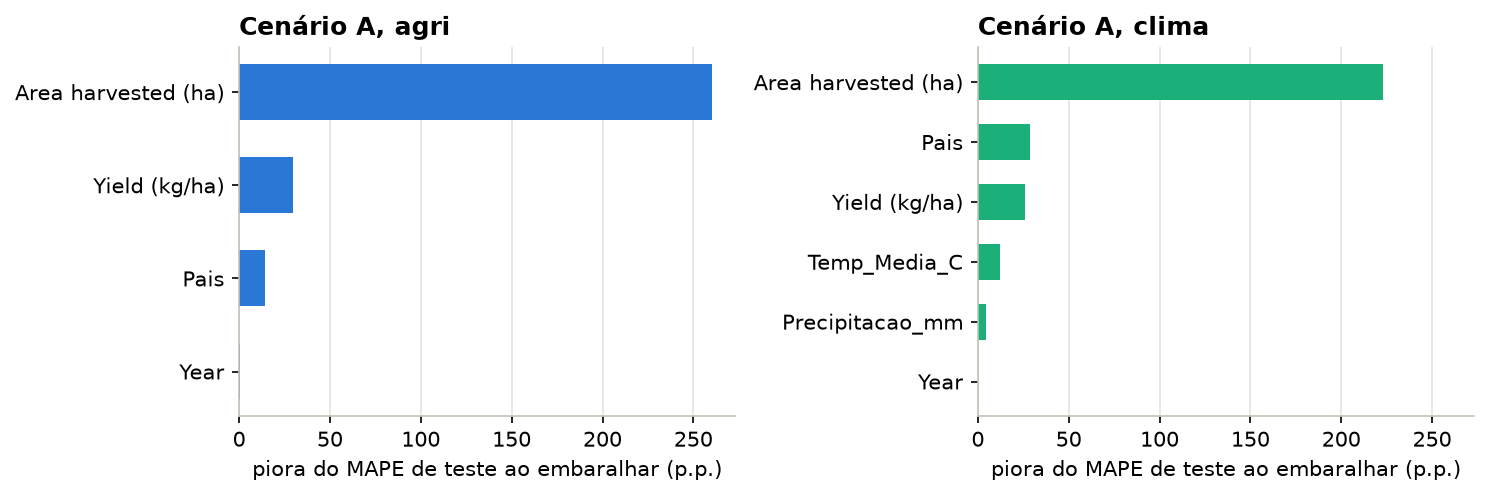
\includegraphics[width=\linewidth]{importancia_atributos.png}
\caption{Importância por permutação no teste: piora do MAPE ao embaralhar cada atributo (Cenário A).}
\label{fig:importancia}
\end{figure}

\paragraph{Baseline manual.} Uma Regressão Linear padronizada (\texttt{StandardScaler} e
\textit{one-hot} do país), no mesmo split, obteve MAPE de 24,3\% (agrícola) e 25,0\% (com
clima). É a mesma ordem da Regressão Linear agrícola do artigo, mas muito distante dos 2,13\%
reportados para o cenário com clima.

\subsubsection{Sensibilidade ao preset e ao tempo}
\label{sec:sensibilidade}

A Tabela~\ref{tab:sensibilidade} compara três presets com orçamentos de 30, 60 e 120\,s no
Cenário A agrícola.
\begin{itemize}
  \item \textbf{\texttt{best\_quality} e \texttt{high\_quality}} melhoram com o tempo: com
  30\,s mal começam o \textit{stacking}, e com 120\,s chegam a cerca de 7\%.
  \item \textbf{\texttt{medium\_quality}}, sem \textit{bagging}, termina em cerca de 22\,s e
  teve o menor MAPE de teste nesta execução (6,05\%). Essa diferença é menor que a variação
  entre sementes do próprio \texttt{best\_quality} (6,0\% a 8,1\%).
\end{itemize}
O preset não foi escolhido pelo teste, o que seria usar o teste para selecionar o modelo.
Mantivemos o \texttt{best\_quality} com 120\,s, que valida todos os modelos fora da amostra:
é a estimativa mais confiável com 120 linhas de treino.

\begin{table}[H]
\centering
\caption{Sensibilidade ao preset e ao \texttt{time\_limit} (Cenário A, agrícola): MAPE de teste (\%).}
\label{tab:sensibilidade}
\begin{tabular}{@{}lrrr@{}}
\toprule
Preset & 30\,s & 60\,s & 120\,s \\
\midrule
\texttt{medium\_quality} & 6,05 & 6,05 & 6,05 \\
\texttt{high\_quality} & 11,66 & 8,75 & 7,11 \\
\texttt{best\_quality} & 11,54 & 8,54 & 7,20 \\
\bottomrule
\end{tabular}
\end{table}

\paragraph{Variabilidade entre sementes.} Com as sementes 42, 7 e 2026, o MAPE de teste do
Cenário A foi de $7{,}12 \pm 1{,}06$\% (agrícola) e $8{,}09 \pm 1{,}06$\% (com clima). Diferenças
abaixo de cerca de 1 ponto percentual não são conclusivas com 36 pontos de teste.

\subsection{Desempenho preditivo}

No Cenário A, o modelo agrícola tem R\textsuperscript{2} de 0,994. O erro por ano é de 5,0\%
em 2021, 10,2\% em 2022 e 6,4\% em 2023. A Figura~\ref{fig:mape-pais} mostra o MAPE por
país: Chile, Suriname, Uruguai e Equador concentram os maiores erros, e Chile e Suriname
dobram de erro com clima. São países de produção menor ou mais variável, o mesmo padrão
relatado no artigo original e uma limitação conhecida do MAPE.

\begin{figure}[H]
\centering
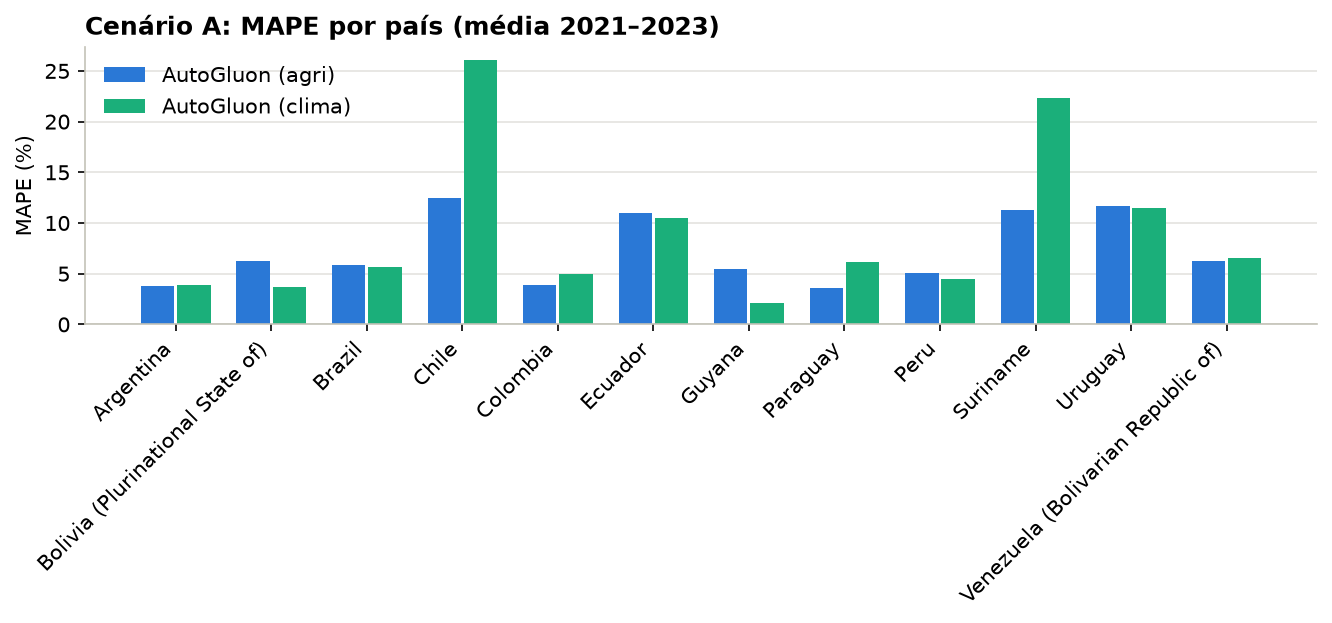
\includegraphics[width=0.85\linewidth]{mape_por_pais_A.png}
\caption{MAPE do AutoGluon por país (Cenário A, média 2021--2023).}
\label{fig:mape-pais}
\end{figure}

\section{Comparação com o artigo original}

A Tabela~\ref{tab:comparacao} e a Figura~\ref{fig:comparacao-final} consolidam o MAPE do
AutoGluon e dos modelos manuais do artigo original nos quatro cenários.

\begin{table}[H]
\centering
\caption{Comparação de MAPE (\%): AutoGluon (AutoML) versus modelos manuais do artigo original.}
\label{tab:comparacao}
\begin{tabular}{@{}llrrrr@{}}
\toprule
Cenário & Atributos & LR & SVR & XGBoost & AutoGluon \\
\midrule
Holdout 2021--2023 & agrícolas & 32,38 & 121,15 & 13,72 & \textbf{7,20} \\
Holdout 2021--2023 & + clima & \textbf{2,13}\textsuperscript{*} & 13,00\textsuperscript{*} & 8,79\textsuperscript{*} & 8,99 \\
CV $k=5$ & agrícolas & 34,87 & 137,23 & 12,47 & \textbf{5,05} $\pm$ 0,48 \\
CV $k=5$ & + clima & 34,60 & 121,00\textsuperscript{\dag} & 11,30 & \textbf{6,55} $\pm$ 1,29 \\
\bottomrule
\end{tabular}
\\[2pt]
\footnotesize{\textsuperscript{*}Ver aproximação na Tabela~\ref{tab:baseline-artigo}.
\textsuperscript{\dag}O artigo relata apenas ``superior a 120\%'' para este valor.}
\end{table}

\begin{figure}[H]
\centering
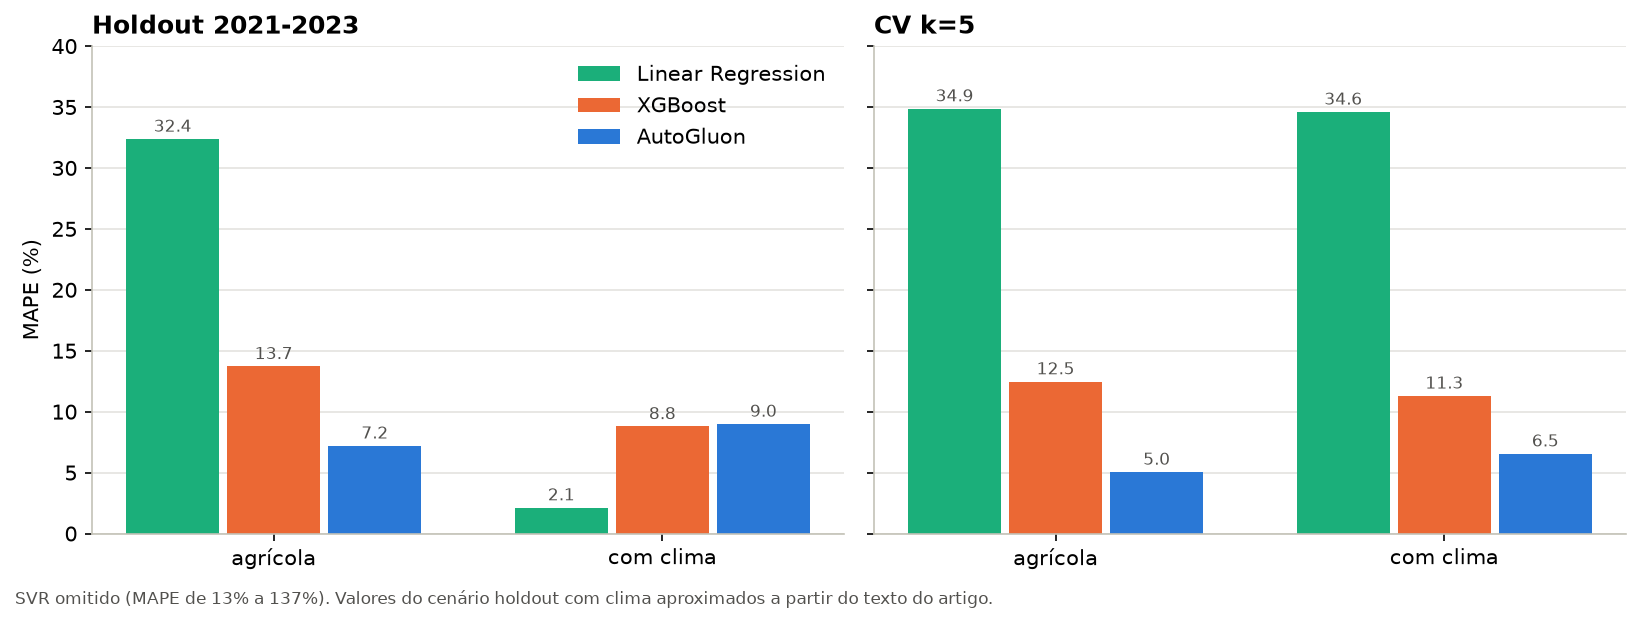
\includegraphics[width=\linewidth]{comparacao_final.png}
\caption{MAPE do AutoGluon versus modelos manuais do artigo original, por cenário (SVR omitido).}
\label{fig:comparacao-final}
\end{figure}

O AutoGluon supera o XGBoost manual em três cenários:
\begin{itemize}
  \item no holdout agrícola, com quase metade do erro (7,20\% contra 13,72\%);
  \item na validação cruzada, nos dois conjuntos de atributos, com menos da metade do erro.
\end{itemize}
No holdout com clima, fica empatado com o XGBoost e atrás da Regressão Linear do artigo.
Esses dois valores, porém, são aproximações extraídas do texto, e o 2,13\% da Regressão
Linear não se reproduz com uma Regressão Linear padronizada nos mesmos dados (cerca de 25\%).

\section{Discussão crítica}

\paragraph{Vantagens.}
\begin{itemize}
  \item Não há busca manual de modelo nem de hiperparâmetros: as decisões do grupo se
  resumem ao preset e ao orçamento de tempo, ambos justificados empiricamente.
  \item O \textit{bagging} e o \textit{stacking} trouxeram ganhos consistentes mesmo com 120
  linhas de treino.
  \item A ferramenta é auditável: o \textit{leaderboard} com erro de teste por modelo, os
  pesos do ensemble e a importância por permutação permitem entender a solução.
\end{itemize}

\paragraph{Custo computacional.} O Cenário A leva cerca de 2 minutos por conjunto de
atributos. O notebook completo, com 24 treinos (incluindo sensibilidade, sementes e
validação cruzada), leva cerca de 30 minutos numa CPU de notebook. A predição é
instantânea.

\paragraph{Limitações.}
\begin{itemize}
  \item \textbf{Teste pequeno.} São 36 pontos de teste, e a variação entre sementes tem a
  mesma ordem das diferenças entre presets.
  \item \textbf{Semente parcial.} A semente variou os modelos, mas não a divisão dos folds
  do \textit{bagging}.
  \item \textbf{Clima não ajudou.} As variáveis climáticas pioraram levemente o resultado
  nos dois cenários, ao contrário do que o artigo sugere para países com maior
  variabilidade climática.
  \item \textbf{Menos interpretável.} O ensemble final é menos interpretável que um único
  XGBoost: a inspeção mostra a sua composição, mas não uma regra simples.
  \item \textbf{Validação cruzada otimista.} A validação cruzada aleatória (Cenário B)
  mistura anos e é mais otimista que o holdout temporal. A limitação também vale para o
  artigo, que usa o mesmo protocolo.
\end{itemize}

\section{Conclusão}

Usamos os dados e a configuração experimental do artigo original e automatizamos a seleção
de modelos, os hiperparâmetros e a combinação deles. Comparando por MAPE, o AutoGluon
superou o XGBoost manual em três dos quatro cenários replicados e empatou no quarto. Ficou
sempre à frente do SVR e, exceto no holdout com clima, da Regressão Linear.

A inspeção do processo mostrou de onde vem o ganho: do ensemble com \textit{bagging} e
\textit{stacking}, com o Extra Trees como base, e não de hiperparâmetros especiais. A área
colhida é, de longe, o atributo mais informativo.

Como próximos passos, sem exigir dados adicionais, ficam:
\begin{itemize}
  \item variar também a divisão dos folds;
  \item usar uma validação temporal dentro do AutoGluon, para que a seleção de modelos
  reflita a previsão do futuro;
  \item testar a generalização por país com leave-one-country-out.
\end{itemize}

\bibliographystyle{plainnat}
\bibliography{referencias}

\end{document}
